\section{LLM Serving}
\label{chap:background:sec:serving}

LLM serving refers to the process of deploying a Large Language Model (LLM) to handle inference requests.
The memory and computation requirements of LLM inference make this process particularly challenging, necessitating dedicated optimizations, parallelization strategies, and hardware acceleration. In this section, we cover the primary optimization techniques used to accelerate LLM inference.

\subsection{KV Caching}

LLMs operate as next-token predictors: given an input prompt, they generate text autoregressively by producing one token at a time. The model outputs a probability distribution over the next token, samples from it, appends the selected token to the context, and repeats this process. The first token is generated solely from the prompt, while each subsequent token is produced using both the original prompt and all previously generated tokens. This sequential dependency makes efficient reuse of past computations essential.

KV caching is a key optimization that enables this efficiency. During attention, each token produces a query, key, and value projection ($\vec{q}_i$, $\vec{k}_i$, $\vec{v}_i$). KV caching stores the keys and values computed for all previously processed tokens so that, when generating a new token, the model only needs to compute its own projections while reusing the cached $k_1,\dots,k_{i-1}$ and $v_1,\dots,v_{i-1}$. This greatly reduces redundant computation, especially for long sequences.

KV caching also delineates the two distinct phases of LLM inference:

\begin{itemize}
    \item \textbf{Prefill Phase}: The model processes all prompt tokens in parallel, computing their $K$ and $V$ projections and populating the KV cache. This phase typically generates the first output token and is predominantly \emph{compute-bound}.
    
    \item \textbf{Decode Phase}: The model then generates tokens one by one. Only the most recently generated token is fed into the model, while the cached keys and values from earlier tokens are reused to avoid recomputation. Because each decoding step requires reading ever-growing KV caches, this phase is generally \emph{memory-bound}.
\end{itemize}


\subsection{Chunk Prefill and Continuous Batching}

Modern LLM inference systems, such as vLLM \cite{kwon2023efficient}, employ a flexible scheduling method known as continuous batching, in which multiple sequences are processed together. Individual sequences are replaced with new ones whenever a sequence either reaches its maximum length or emits an end-of-sequence token. This approach is enabled by chunked prefill, which splits the prefill phase into several smaller chunks. By processing chunks of tokens rather than a full prompt, the system can interleave prefill and decode operations across multiple sequences in parallel, improving throughput without unduly increasing decoding latency.

\subsection{PagedAttention}

Another significant optimization employed in vLLM \cite{kwon2023efficient} is \textbf{PagedAttention}. This method leverages the principles of virtual memory paging to manage KV caches more flexibly: instead of requiring a single, large, contiguous memory allocation, PagedAttention enables the cache to reside in non-contiguous physical memory pages. A memory manager dynamically allocates new pages as the KV cache grows and frees pages once a sequence finishes. Moreover, in cases where multiple sequences share a common prefix, the pages storing that prefix can be mapped to and shared among those sequences (via copy-on-write and reference counting).

\subsection{Quantization}

Quantization is a widely used technique to accelerate compute-intensive applications. It involves converting floating-point values into lower-bit-width formats, sacrificing a small amount of accuracy for increased computational efficiency. As discussed in Chapter \ref{chap:methods:sec:model}, quantization affects performance in two main ways. First, it reduces the volume of data transferred from memory to processors. Second, when specialized functional units are used, they enable simpler and faster arithmetic operations compared to standard floating-point addition and multiplication units.

Floating-point formats are composed of three components: the sign bit, which indicates whether the number is positive or negative, the exponent bits, and the mantissa bits. The value of a floating-point number is given by the formula
$(-1)^S \cdot 2^{\text{exp} - \text{bias}} (1 + \text{mantissa})$.
The number of exponent bits determines the range of representable values, while the mantissa bits define the precision within that range.
Figure \ref{fig:floating} illustrates six popular floating-point formats used in modern AI accelerators, highlighting their sign, exponent, and mantissa fields.

LLMs are typically trained using 16-bit floating-point formats, such as bfloat16 (Brain Float 16) precision (8 bits for the exponent and 7 bits for the mantissa), or FP16 (5 bits for the exponent and 10 bits for the mantissa). Consequently, open-source models are available in that format, and most accelerators and inference engines support these types. Recently, AI accelerators have begun supporting quantization to 8-bit floating-point formats, further alleviating memory pressure and reducing the computational cost of inference.

\begin{figure}[h!]
    \centering
    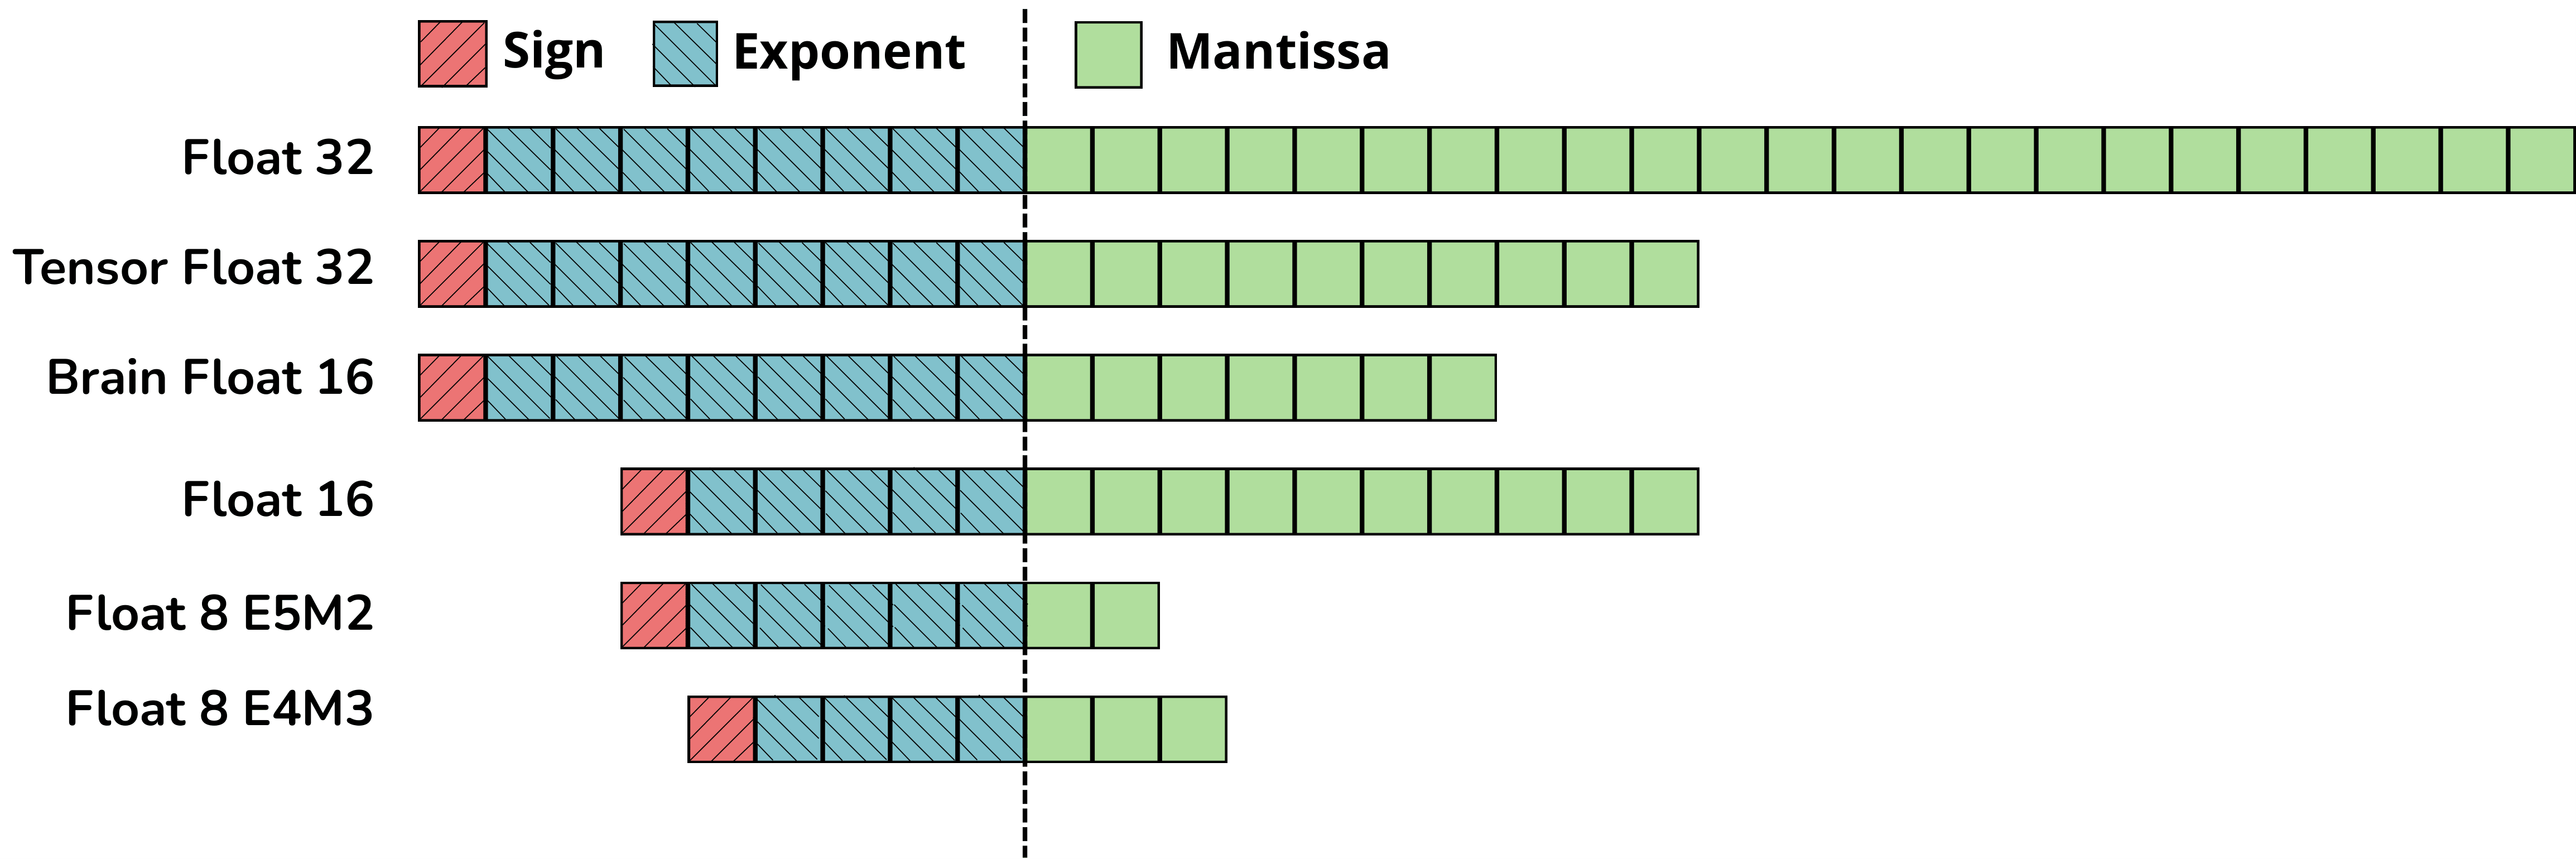
\includegraphics[width=\textwidth]{figs/Precision with hatch.pdf}
    \caption{Mixed Precision Floating-Point formats.}
    \tagpdfsetup{alttext={Mixed Precision Floating-Point formats.}}
    \label{fig:floating}
\end{figure}

Currently, two main types of FP8 quantization are used: W8A16 (8-bit weights and 16-bit activations) and W8A8 (8-bit weights and 8-bit activations). In particular, W8A8 typically employs the E4M3 format (4 exponent bits and 3 mantissa bits) for weights, and the E5M2 format (5 exponent bits and 2 mantissa bits) for activations. These two approaches target different hardware configurations. The former utilizes dedicated FP8 functional units to accelerate computation, while the latter is designed for hardware that only supports half-precision operations but still benefits from reduced memory usage.
Other quantization methods exist, but they fall outside the scope of this evaluation.

\subsection{Multi-GPU Inference}
\label{chap:background:sec:multigpu}

Growing model sizes and throughput requirements frequently exceed the memory and compute capacity of a single device, motivating multi-GPU strategies that distribute computation at the cost of increased communication. A variety of parallelism techniques have therefore been developed to balance memory capacity, communication overheads, and GPU utilisation.

\begin{figure}[h!]
    \centering
    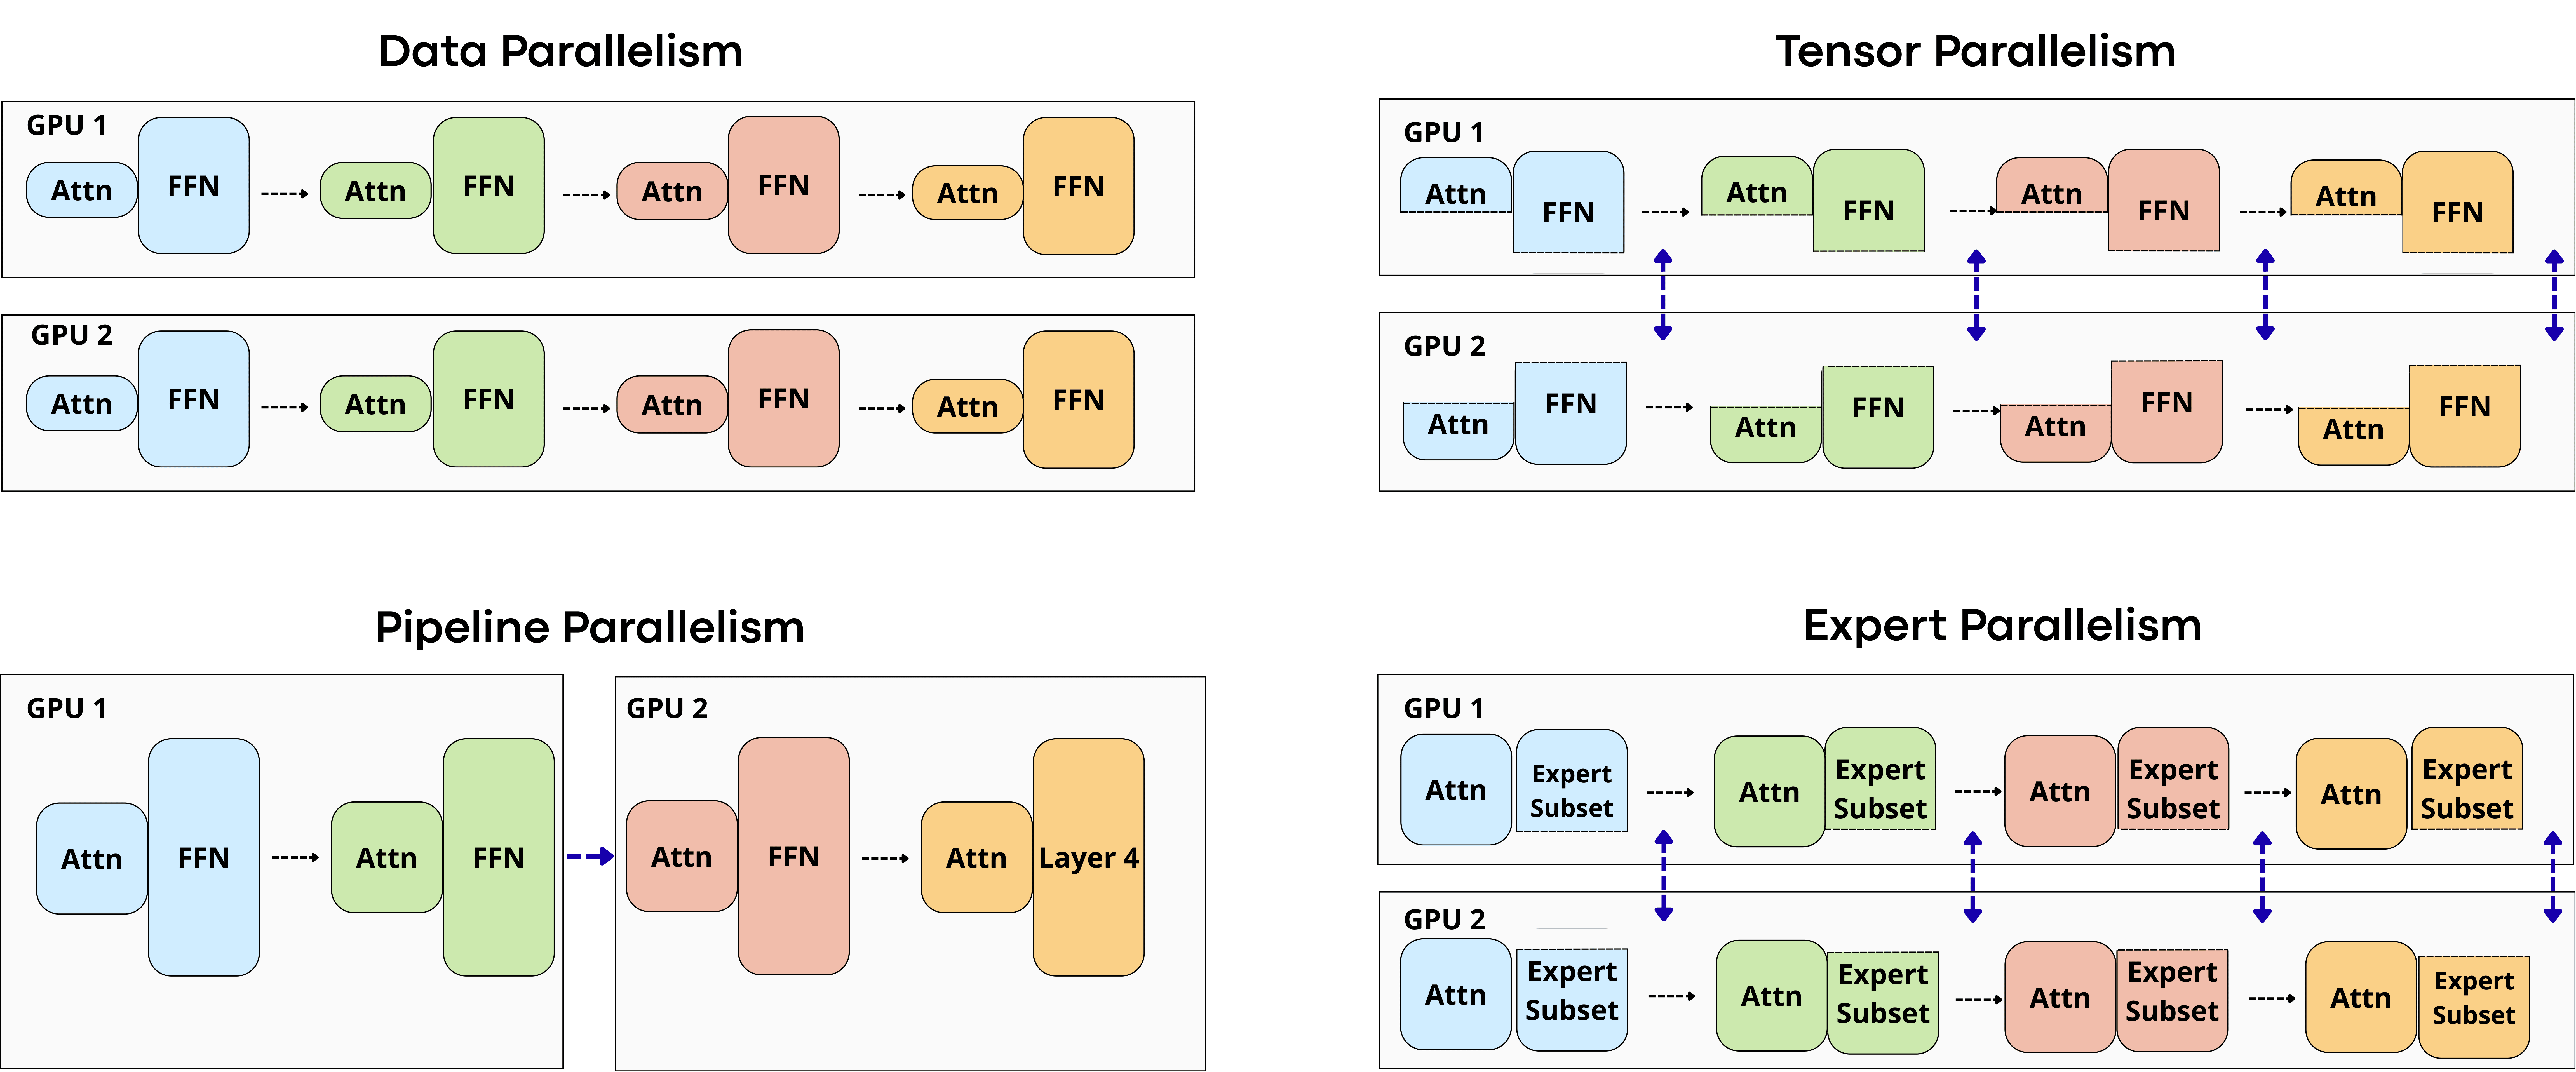
\includegraphics[width=0.95\textwidth]{figs/parallelism.pdf}
    \vspace{5mm}
    \caption{Comparison of multi-GPU techniques.}
    \tagpdfsetup{alttext={Comparison of multi-GPU techniques.}}
    \label{fig:parallel}
\end{figure}

\begin{itemize}
    \item \textbf{Data Parallelism (DP)} launches multiple independent model replicas on separate GPUs to increase serving throughput. Because each replica contains the full set of parameters, DP does not increase the effective memory available to a single model instance, but it scales well and requires no inter-GPU communication during inference.

    \item \textbf{Pipeline Parallelism (PP)} partitions the model’s layers across GPUs. Each device executes a contiguous block of layers and forwards intermediate activations to the next device. This expands the memory capacity accessible to a single model instance while introducing only moderate communication overhead.

    \item \textbf{Tensor Parallelism (TP)} shards parameters within each layer—such as attention heads and feed-forward weights—across multiple GPUs. This provides a finer-grained way to increase total available memory and keep all devices active, at the cost of frequent collective operations (e.g., all-gather).

    \item \textbf{Expert Parallelism (EP)} distributes the experts in Mixture-of-Experts layers across devices, allowing each GPU to store only a subset of expert parameters. Non-expert components—such as attention projections, layer norms, and routing modules—remain replicated on all devices. As a result, EP increases effective memory capacity primarily for expert-heavy layers while leaving the rest of the model duplicated.
\end{itemize}